\documentclass[tikz]{standalone}
\usepackage{pgfplots}
\pgfplotsset{compat=1.15}
\usepackage{mathrsfs}
\usetikzlibrary{arrows,calc}
\usepackage{tkz-euclide}

\pagestyle{empty}

\definecolor{AngleClr}{rgb}{0,0.39215686274509803,0}
\definecolor{ShapeClr}{rgb}{0.6,0.2,0}

\begin{document}

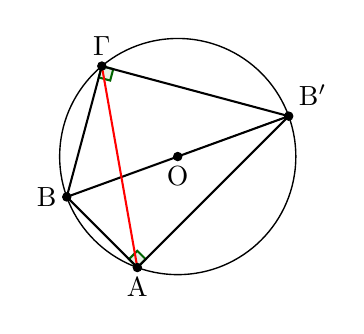
\begin{tikzpicture}[scale=.75]
\tkzSetUpLine[line width=1pt,color=black]
\tkzSetUpPoint[fill=black]

\tkzDefPoints{0/0/O}

\tkzDefPoint(20:2){X}
\tkzDefPoint(130:2){C}
\tkzDefPoint(-160:2){B}
\tkzDefPoint(-110:2){A}

\tkzDrawCircle[color=black,fill=white,line width=0.5pt](O,X)

\tkzMarkRightAngles[line width=0.75pt, size=.2,color=AngleClr,fill=AngleClr,fill opacity=0.1](B,A,X B,C,X)

\tkzDrawSegments[line width=0.75pt,color=black](A,B B,C C,X A,X B,X)
\tkzDrawSegments[line width=0.75pt,color=red](A,C)
\tkzDrawSegments[line width=0.5pt,color=black,dashed,dash pattern=on 1pt off 1.75pt](O,X)

\tkzDrawPoints[size=3](A,B,C,O,X)

\tkzLabelPoint[below](A){$\rm A$}
\tkzLabelPoint[left](B){$\rm B$}
\tkzLabelPoint[above](C){$\rm \Gamma$}
\tkzLabelPoint[above right](X){$\rm B'$}
\tkzLabelPoint[below](O){$\rm O$}


\end{tikzpicture}
\end{document}
